\hypertarget{uppgifter-puxe5-svenska}{%
\section{Uppgifter (på svenska)}\label{uppgifter-puxe5-svenska}}

\begin{enumerate}
\item
  Undersöker följande replicator ekvation

  \[\begin{aligned}
   \dot{x}(t)  =   x(t) (1-x(t)) (1/4 - 1/2 x(t)) 
  \end{aligned}\]

  Hitta alla jämviktspunkter och använder linjärisering för att bestäm
  stabilitet. Har modellen dynamik som mest likna prisoners dilemna,
  stag hunt eller hawk-dove?
\item
  SI modellen av en epidemi har följande tillståndsform

  \[\frac{dS}{dt}  =  - \beta S I +  \gamma I\]

  Antar att \(\beta=1/3\), \(\gamma=1/6\) och \(S+I=1\).

  \begin{itemize}
  \tightlist
  \item
    Visa att det finns en jämviktspunkt där \(S_*=I_* = 1/2\)
  \item
    Bestäm stabiliteten av jämviktspunkten.
  \item
    Om \(\beta=1/3\) för vilket värde av \(\gamma\) är jämviktspunkten
    där \(S_* = 1\) stabil?
  \end{itemize}
\item
  Följande tillstånds model beskriver tillväxt av fisk bestånd i en sjö,
  där \(x(t)\) är tusentals fisk i sjön.

  \[\begin{aligned}
    \frac{d}{dt}x(t) = r x(t)(1- x(t)) + c 
  \end{aligned}\]

  där \(c>0\) är inflödet av nya fisk (från en närliggande sjö) och
  \(r>0\) är tillväxthastighet.

  \begin{itemize}
  \tightlist
  \item
    Hitta alla jämviktspunkter \(x_*\) till ekvationen och beräkna
    stabiliteten.
  \item
    Hur många fisk finns i sjön när \(t \rightarrow \infty\) om modellen
    stämmer?
  \end{itemize}
\item
  När det finns minst \(F = 100\) fisk i sjön utförs fisketillstånd så
  att turister får kommer dit och fiskar. Sjömyndigheten har kommit fram
  till att följande model gäller i detta fall.

  \[\begin{aligned}
    \frac{dx}{dt} = f(x) = r x(1- x) + c - b \frac{x^3}{F^3 + x^3}
  \end{aligned}\]

  De skatar parameter \(r\), \(b\), \(c\) och \(F\) och skissa
  funktionen, \(f(x)\), nedan.

  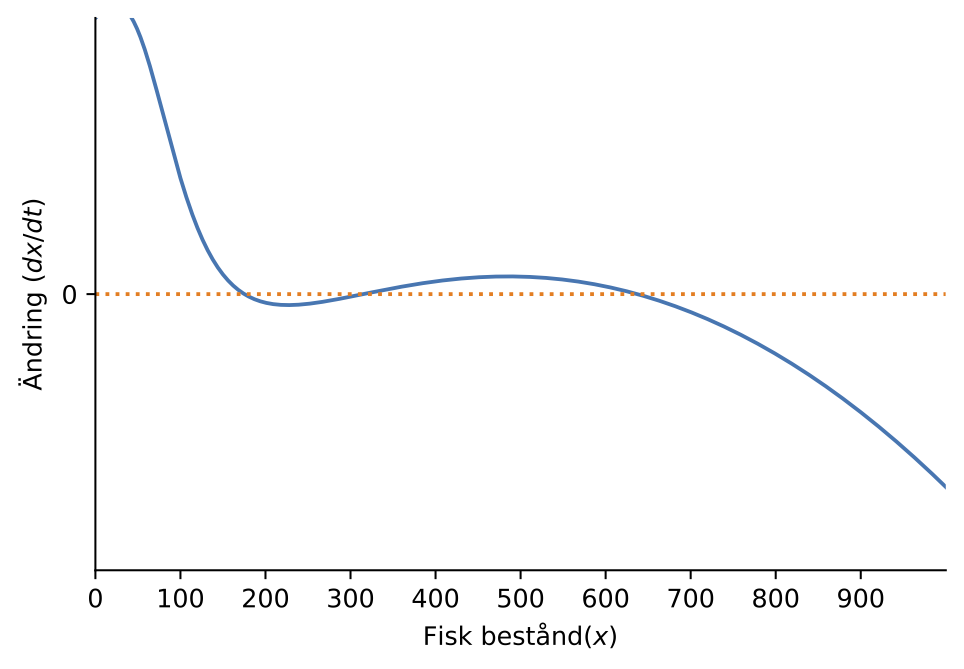
\includegraphics[width=4.16667in,height=\textheight]{../images/lesson1/fisk.png}

  Hur många jämviktspunkter har \(f(x)\)? Hur många är stabila? Hur kan
  man tolka modellen när det gäller långsiktig fisk beståndet i sjön?

  \textbf{Obs:} Använd grafen att lösa problemet! Du behöver inte lösa
  ekvationen.
\end{enumerate}
